% ----------------------------------------------------------------------------------------------------- %
% Relatório 2 de PDS - Baseado na classe UFTeX
% ----------------------------------------------------------------------------------------------------- %

\documentclass[tcc]{classe_uftex/uftex}
% ---- Esse comando cria o nome uftex estilizado
\newcommand\uftex{UF\TeX}

\usepackage{lipsum}
\usepackage{tikz}
\usepackage[siunitx]{circuitikz}
\usetikzlibrary{arrows}

\usepackage[alf,abnt-emphasize=bf]{referencias_abnt/abntex2cite}
\usepackage{xcolor}
\usepackage{mathptmx} % Times New Roman (ABNT)
\usepackage{float}

\renewcommand{\lstlistingname}{Código}
\renewcommand{\lstlistlistingname}{Lista de Códigos}

\definecolor{codegreen}{rgb}{0,0.6,0}
\definecolor{codegray}{rgb}{0.5,0.5,0.5}
\definecolor{codepurple}{rgb}{0.58,0,0.82}
\definecolor{backcolour}{rgb}{0.98,0.98,0.98}
\definecolor{codeblue}{rgb}{0,0,0.8}

\lstset{
  language=Matlab,
  backgroundcolor=\color{backcolour},   
  commentstyle=\color{codegreen},
  keywordstyle=\color{codeblue}\bfseries,
  numberstyle=\normalsize\color{codegray},
  stringstyle=\color{codepurple},
  basicstyle=\ttfamily\small\color{black},
  breakatwhitespace=false,         
  breaklines=true,                 
  captionpos=b,                    
  keepspaces=true,                 
  numbers=left,                    
  numbersep=12pt,                  
  showspaces=false,                
  showstringspaces=false,
  showtabs=false,                  
  tabsize=2,
  frame=lines,
  rulecolor=\color{black!30},
  xleftmargin=20pt,
  framexleftmargin=5pt,
  aboveskip=20pt,
  belowskip=20pt
}

\renewcommand{\backrefpagesname}{}
\renewcommand{\backref}{}
\renewcommand*{\backrefalt}[4]{}

% ---- Ajuste para transformar a capa de TCC em Relatório e numeração no rodapé
\makeatletter
\renewcommand*{\ps@plain}{%
  \let\@mkboth\@gobbletwo
  \let\@oddhead\@empty
  \def\@oddfoot{%
    \reset@font
    \hfil
    \thepage
  }%
  \let\@evenhead\@empty
  \let\@evenfoot\@oddfoot
}

\renewcommand\frontpage@maintext{
  \sloppy\nohyphens{Relatório de Laboratório apresentado à disciplina de Processamento Digital de Sinais do curso de \local@deptname\ da \local@universityname .

 \vspace{.5cm}
  \nohyphens{%
    \count1=0
    \@whilenum \count1<\@advisor \do{%
    \ifcase\count1 % same as \ifnum0=\count1
        Professor: \csname uftAdvisorDegree:\the\count1 \endcsname \ 
        \csname uftAdvisorName:\the\count1 \endcsname \ 
        \csname uftAdvisorSurname:\the\count1 \endcsname \ \par
    \else
        \local@coadvisorstring: \csname uftAdvisorDegree:\the\count1 \endcsname \ 
        \csname uftAdvisorName:\the\count1 \endcsname \ 
        \csname uftAdvisorSurname:\the\count1 \endcsname \ \par
    \fi
    \advance\count1 by 1}
  } \par
}
}
\makeatother

% ---- Início do documento
\begin{document}
  % ---- Descrição do título do trabalho 
  \title{Relatório 2 de PDS: Operações com Sequências}
  % ---- Nome do autor ou autores do trabalho
  \author{Maurício}{Moura de Carvalho}
  % ---- Nome do orientador do trabalho.
  \advisor{Prof.}{Ivan}{Ney Alvizuri Romani}{Dr.}

  % ---- Departamento
  \department{EE} % ou o departamento correto
  
  % ---- Data
  \date{15}{04}{2026}
  
  % ---- Palavras-chaves
  \keyword{Processamento Digital de Sinais}
  \keyword{Sinais Discretos}
  \keyword{Octave}

  % ---- Palavras-chaves em inglês
  \foreignkeyword{Digital Signal Processing}
  \foreignkeyword{Discrete Signals}
  \foreignkeyword{Octave}
  
  \maketitle
  \frontmatter

  % ---- Cria o sumário
  \tableofcontents 
  
  % --- Marca o inicio dos elementos textuais
  \mainmatter
  \setcounter{page}{1} % Corrige bug da página 0 no uftex (zref chap:first não definido)
  \onehalfspacing

% ----------------------------------------------------------------------------------------------------- %
% Capítulos do trabalho
% ----------------------------------------------------------------------------------------------------- %

\chapter{Introdução}

Este relatório tem como objetivo apresentar os resultados obtidos no segundo laboratório da disciplina de Processamento Digital de Sinais (PDS), cujo tema central está nas formas de \textbf{Operações com Sequências}.

Nesta prática, explorou-se a geração e plotagem de sinais discretos no tempo, bem como operações matemáticas entre eles, através de rotinas desenvolvidas na ferramenta Octave \cite{octaveman}. As atividades seguiram as diretrizes do roteiro de laboratório \cite{roteiro02} e fundamentaram-se na literatura clássica de processamento de sinais como Oppenheim e Willsky \cite{oppenheim_willsky}, Proakis e Manolakis \cite{proakis_manolakis} e Ingle \cite{ingle2017}.

O desafio desta prática consistiu em modelar manualmente a geração das funções basilares, como o \emph{impulso unitário} e o \emph{degrau unitário}, bem como as próprias operações entre vetores de sinais discretos, garantindo-se assim a plena absorção da lógica de programação que fundamenta as equações de processamento de sinais discretos. No desenvolvimento destas rotinas, valeu-se puramente do software Octave, implementado através de códigos de alto nível construídos passo a passo sem dependências simplificadoras para enrijecer a compreensão sobre limites, tamanhos de vetores, deslocamento da base de tempo ($n$) e alinhamento do escopo na sobreposição de sinais.

\chapter{Metodologia e Procedimentos Práticos}

\section{Parte I - Implementação Manual de Funções}
Criou-se customizadamente as funções essenciais que operam atreladas a um vetor temporal com limite inferior e superior explícitos ($n1 \le n \le n2$).

As funções criadas e suas assinaturas foram organizadas em arquivos independentes:
\begin{itemize}
    \item[\textbf{a)}] \texttt{seq\_imp}: Gera uma função impulso deslocada no instante $n_0$.
    \item[\textbf{b)}] \texttt{seq\_degrau}: Gera uma função degrau discreta a partir de $n_0$.
    \item[\textbf{c)}] \texttt{soma\_sinais}: Alinha dois vetores definidos em intervalos $n$ possivelmente disjuntos, preenchendo áreas não-concorrentes com zeros, e efetua a adição ponto a ponto sobre o \emph{overlap} esticado resultante.
    \item[\textbf{d)}] \texttt{mult\_sinais}: Utiliza o mesmo mecanismo lógico de esticamento temporal com \emph{zero-padding} intrínseco, porém efetuando o produto ponto a ponto das sequências.
    \item[\textbf{e)}] \texttt{shift\_sinais}: Promove o deslocamento vetorial temporal mapeando os valores frente a um coeficiente $n_0$.
\end{itemize}


\section{Parte II - Geração e Plotagem com Intervalo Sinalizado}
Utilizando as novas instâncias procedurais da \emph{Parte I}, foram montadas as formulações relativas aos sinais:
\begin{enumerate}
    \item[\textbf{a)}] $x[n] = 2\delta[n + 2] - \delta[n - 4], -10 \leq n \leq 10$
    \item[\textbf{b)}] $x[n] = n[u(n) - u(n - 10)] + [u(n - 10) - u(n - 20)]10e^{-0.3(n-10)}, \ 0 \leq n \leq 40$
\end{enumerate}

\section{Parte III - Operações e Rebatimento sobre a Sequência Fixa}
Dada a sequência declarativa inicial $x[n] = \{1,2,3,4,5,6,7,6,5,4,3,2,1\}$, as composições criadas foram determinadamente plotadas considerando um espaçamento vetorial originário, simuladas em escopo finito:
\begin{enumerate}
    \item[\textbf{a)}] $x_1[n] = 0,5x[n - 3] - 2x[n + 2]$
    \item[\textbf{b)}] $x_2[n] = x[2 - n] + x[n]x[n + 2]$
\end{enumerate}

Nota-se a importância da abordagem reflexiva temporal de indexação invertida que se faz presente pela presença do termo condicional rebatido em amplitude $x[2-n]$.

\section{Parte IV - Sinal Complexo Exponencial Expandido}
Ao final da demanda laboratorial, gerou-se o sinal discreto de natureza complexa modelado por uma parte resistiva/atenuadora e uma reativa/oscilatória aglutinadas num mesmo argumento polar:
\begin{equation}
    x[n] = e^{(-0,2+j0,3)n} , -25 \leq n \leq 25 \nonumber
\end{equation}
Fez-se necessário plotar isoladamente sob uma mesma janela gráfica (\texttt{subplot}) quatro características da função: Magnitude, Fase, Parte Real e Parte Imaginária.

\chapter{Resultados e Códigos Fontes}

\textit{Cada script implementado originou sua respectiva resposta gráfica, as quais são demonstradas passo a passo nessa secção.}

\section{Parte I: Funções de Suporte (Octave)}

A função \texttt{seq\_imp(n0, n1, n2)} cria um vetor baseado num argumento lógico para representar o Delta de Dirac discreto:
\lstinputlisting[language=Matlab, caption={{Função de criação do Impulso Unitário.}}]{codigos/seq_imp.m}

A função \texttt{seq\_degrau(n0, n1, n2)} repete a natureza lógica anterior, estendida para abranger desde $n_0$ até o último índice validado:
\lstinputlisting[language=Matlab, caption={{Função de criação do Degrau Unitário.}}]{codigos/seq_degrau.m}

A função \texttt{soma\_sinais(x1, n1, x2, n2)} engloba um redimensionamento dinâmico do eixo do tempo limitante entre os menores extremos inferiores e os absolutos limites superiores de ambas as sequências, utilizando atribuição lógica (logical indexing) tolerada pelo software:
\lstinputlisting[language=Matlab, caption={{Função Soma entre Sequências.}}]{codigos/soma_sinais.m}

Acompanhando esse formato de sobreposição forçada, obteve-se êxito análogo com a função \texttt{mult\_sinais}:
\lstinputlisting[language=Matlab, caption={{Função de Multiplicação de Sequências.}}]{codigos/mult_sinais.m}

E por fim, \texttt{shift\_sinais(x, n, n0)} desloca as instâncias atrasando ou adiantando os tempos associados à forma do vetor numérico de origem:
\lstinputlisting[language=Matlab, caption={{Função Deslocamento no Tempo.}}]{codigos/shift_sinais.m}

\section{Parte II: Utilização Plena na Base de Tempos}

\lstinputlisting[language=Matlab, caption={{Composição 2a e 2b.}}]{codigos/parte2.m}

\subsection*{a) Função em Delta Duplo}
\begin{figure}[H]
\centering

\includegraphics[width=0.8\textwidth]{figuras/parte2_a.png}
\caption{Parte II a) 2Deltas deslocados.}\label{fig:p2a}
\end{figure}

\subsection*{b) Montagem do Decaimento Discreto Intermediário}
A elaboração da função degrau combinada em três janelas demonstra as fronteiras retangulares onde a rampa opera entre $0$ e $10$, e a exponencial de decaimento natural ocorre contida entre $10$ e $20$.
\begin{figure}[H]
\centering

\includegraphics[width=0.8\textwidth]{figuras/parte2_b.png}
\caption{Parte II b) Construção do sinal em três faixas operacionais limitadas por janelas de degrau.}\label{fig:p2b}
\end{figure}

\section{Parte III: Rebatimento e Ampliação Dinâmica}

A execução no script da parte três envolve o uso de reordenamento horizontal prévio a nível elementar de \texttt{arrays} utilizando operações como \texttt{fliplr} e invertendo os índices na modelagem base, providenciando as transformações temporais solicitadas pela variável reversa $x[2-n]$.

\lstinputlisting[language=Matlab, caption={{Processamento de X1 e X2.}}]{codigos/parte3.m}
\begin{figure}[H]
\centering

\includegraphics[width=0.8\textwidth]{figuras/parte3_a.png}
\caption{Item III.a) Operação mista de deslocamento e amplificação escalar.}\label{fig:p3a}
\end{figure}
\begin{figure}[H]
\centering

\includegraphics[width=0.8\textwidth]{figuras/parte3_b.png}
\caption{Item III.b) Gráfico apresentando a incorporação do rebatimento da sequência num somatório sobreposto.}\label{fig:p3b}
\end{figure}

\section{Parte IV: Componentes Ortogonais e Mag/Fase no Plano Z}

Para decompor as propriedades do eixo do número quociente polar \texttt{x = exp((-0.2 + 0.3j) * n)}, evocou-se os extratores clássicos da plataforma (\texttt{real, imag, abs, angle}). Observa-se as oscilações senoidais amortizadas nos quadros ortogonais clássicos de Euler que modelam a respectiva atenuação complexa.

\lstinputlisting[language=Matlab, caption={{Visualização do Comportamento Exponencial Complexo.}}]{codigos/parte4.m}
\begin{figure}[H]
\centering
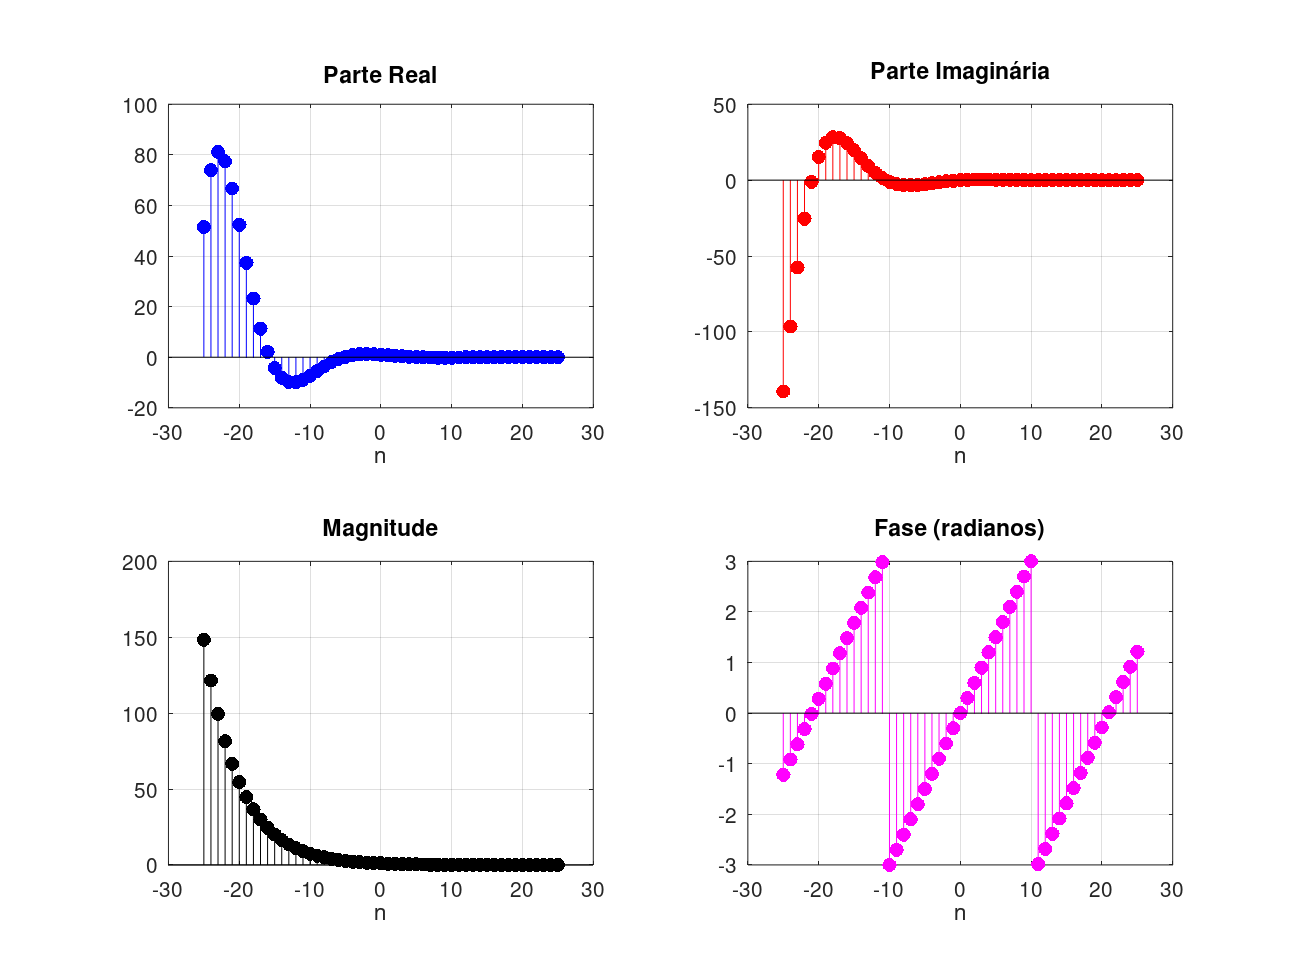
\includegraphics[width=0.85\textwidth]{figuras/parte4.png}
\caption{Decomposição do sinal exponencial complexo amortecido em sub-plotagens.}\label{fig:p4}
\end{figure}


\chapter{Conclusão}

As práticas efetuadas validaram a compreensão profunda das funções de Processamento Digital de Sinais (PDS). A utilização do Octave \cite{octaveman} e a consulta à documentação oficial \cite{matlabdoc} provaram ser ferramentas essenciais para a verificação prática dos conceitos teóricos discutidos em aula e apresentados na literatura técnica consagrada de Proakis \cite{proakis_manolakis} e Oppenheim \cite{oppenheim_willsky}.

As funções escritas manualmente responderam favoravelmente suportando \textit{overlaps} e espaços vazios com atribuição de zeros sem corromper as integridades originais das funções sobre as quais as propriedades comutativas e vetoriais foram executadas. Ademais, as reflexões do plano cartesiano em conjunção da análise tridimensional do número complexo forneceram visualizações riquíssimas para a correlação do campo de fase e de decaimento real. Conclui-se que o domínio da geração e caracterização destes sinais elementares é um passo indispensável para o estudo de sistemas lineares invariantes no tempo (LIT) e transformadas de frequência.

% ----------------------------------------------------------------------------------------------------- %
\backmatter 
\singlespacing   
% ----------------------------------------------------------------------------------------------------- %%%
\bibliography{relatorio_2}

\end{document}
